\topic{Introduction to set theory and \\ functions}{Introduction to set theory and functions}

\subsection{Basic concepts of set theory}
\begin{definition}
    \textbf{(Set).} A set is a collection of objects about which is possible to determine weather or not a particular object is a member of the set.
\end{definition}

Sets are usually denoted by capital letters, and the objects within them are referred to as \textbf{elements}. One way to describe a set is by giving a list of their elements, just as the example below.
\begin{example}
    Let $A$, $B$ and $C$ be three sets such that
    \begin{equation}
        A = \lbrace 1, 2, 3, 4\rbrace \quad\quad\quad B = \lbrace 1, 2, 3, 4\ldots\rbrace \quad\quad\quad C = \lbrace 0, 2, 4, 6\ldots\rbrace
    \end{equation}
\end{example}

Another way to describe a set is by the so called \textbf{set-builder notation}. This notation uses braces to enclose a property that is the qualification for membership in the set.

\begin{example}
    Let $A$ and $B$ be two sets described using the set-builder notation.
    \begin{align}
        A &= \lbrace x\tq x \textrm{ is a natural number } \rbrace = \lbrace 0, 1, 2\ldots\rbrace \\
        B &= \lbrace x\tq x \textrm{ is an even natural number } \rbrace = \lbrace x : 2\tq x \textrm{ and $x$ is natural } \rbrace
    \end{align}
\end{example}

\begin{notation}
    In this previous example, both symbols $\tq$ and $ : $ are used to denote \textit{such as}.
\end{notation}

We write $a\in A$ if $a$ is an element in the set $A$. Otherwise, we write $a\notin A$ to mean that $a$ is not an element in the set $A$. For instance, 2/3 is a rational number, but not an integer one. Then
\begin{equation}
    \frac{2}{3}\in\Q,\quad\textrm{ but } \frac{2}{3}\notin\Z 
\end{equation}

\begin{definition}
    \textbf{(Empty set).} We use $\O$ to refer to the set with no elements, denominated the \textbf{empty set}.
\end{definition}
\begin{definition}
    \textbf{(Subset).} Let $A$ and $B$ be sets. We say that $A$ is a subset of $B$ if every element in $A$ is an element in $B$. If $A$ is a subset of $B$ we write $A\subset B$ and we say \textit{$A$ is contained in $B$} or \textit{$B$ contains $A$}. Otherwise we write $A\notin B$.
\end{definition}
\begin{example}
    Some examples of subsets are
    \begin{align}
        &\N\subset\Z\subset\Q\subset\R\subset\C \\
        &\O\in C\textrm{, where $C$ is any set.} \\
        &A = \{1, 2, 3\} \subset B = \{1, 2, 3, 4, 5\} 
    \end{align}
\end{example}

\begin{definition}
    \textbf{(Equal sets).} Two sets $A$ and $B$ are equal if $A \subset B$ and $B\subset A$; i.e. if they have the same elements.
\end{definition}
\begin{definition}
    We say that $A$ is properly contained in $B$ if $A\subset B$ but $A\neq B$. For example, $\N$ is properly contained in $\Z$ because $\N\subset\Z$, but $\N\neq\Z$.
\end{definition}
\begin{notation}
    We use $:=$ to mean \textit{by definition}. For example, $\N := \{0, 1, 2\ldots\} $.
\end{notation}

\subsection{Power set of a set}
\begin{definition}
    \textbf{(Power set).} Let $A$ be a set. The power set of $A$ is a set whose elements are all the subsets of $A$, and we denote it by $\SP\left( A \right) $
\end{definition}
\begin{example}
    Let $A = \{a, b, c\}$, then the power set of $A$ is
    \begin{equation}
    \SP(A) = \lbrace \O, \{a\}, \{b\}, \{c\}, \{a, b\}, \{a, c\}, \{b, c\}, \{a, b, c\}\rbrace
    \end{equation}
\end{example}

In this previous example, we must keep notice that $\O\in\SP\left( A \right)$ and $\O\subset \SP\left( A \right)$ are not exactly the same thing. In the first one we are refering to the $\O$ element in the set $\SP\left( A \right)$; while in the second, $\O$ is the empty set, which as seen previously is a subset of any set. $\{\O\}\subset \SP\left( A \right)$ has also a different meaning, as $\O$ in this case is the element contained in $\SP\left( A \right)$. We couldn't write $\{\O\}\in \SP\left( A \right)$ because the element $\{\O\}$ is not contained in $\SP\left( A \right) $.

\subsection{Unions and intersections of sets}
\begin{definition}
    \textbf{(Union of sets).} Let $A$ and $B$ be two sets. The union of $A$ and $B$ is another set whose elements are the elements in $A$ and the elements in $B$. We denote this set by $A\cup B$.
    \begin{equation}
        A\cup B := \{x\tq x\in A\textrm{ or } x\in B\}
    \end{equation}
\end{definition}
\begin{example}
    Let $A = \{a, b, c\} $ and $B = \{b, h, f\} $, then
    \begin{equation}
        A\cup B = \{a, b, c, h, f\} 
    \end{equation}
\end{example}
\begin{definition}
    \textbf{(Intersection of sets).} Let $A$ and $B$ be two sets. The intersection of $A$ and $B$ is another set whose elements are the elements that $A$ and $B$ have in common. We denote this set by $A\cap B$.
    \begin{equation}
        A\cap B := \{x\tq x\in A\textrm{ and } x\in B\}
    \end{equation}
\end{definition}
\begin{example}
    Let $A\cap B = \{b\} $ and $C = \{x, y, z\}$, then
    \begin{equation}
        A\cap C = \O \quad\rightarrow\quad\textrm{ we say that $A$ and $C$ are disjoint.}
    \end{equation}
\end{example}

Let $A$, $B$ and $C$ be three non empty sets. The following properties are hold related to the union and intersection operations between those sets.
\newpage
\bgroup
\def\arraystretch{1.5}
\def\tabcolsep{20}
\begin{table}[h!]
\centering
\begin{tabular}{|c|c|}
    \hline
    \textbf{Property name} & \textbf{Properties} \\
    \hline
    Commutativity & $A\cap B = B\cap A$ \\
    \hline
    Commutativity & $A\cup B = B\cup A$ \\
    \hline
    Idempotency & $A\cup A = A$ \\
    \hline
    Idempotency & $A\cap A = A$ \\
    \hline
    Disjoint sets & $A\cap B = \O$ \\
    \hline
    Associativity & $\left( A\cap B \right)\cap C = A\cap\left( B\cap C \right)$ \\
    \hline
    Associativity & $\left( A\cup B \right)\cup C = A\cup\left( B\cup C \right)$ \\
    \hline
    Distributivity & $A\cup\left( B\cap C\right) = \left( A\cup B \right)\cap\left( A\cup C \right)$ \\
    \hline
    Distributivity & $A\cap\left( B\cup C\right) = \left( A\cap B \right)\cup\left( A\cap C \right)$ \\
    \hline
    Cancelation & $A\cup\left( B\cap A \right) = A$ \\
    \hline
    Cancelation & $A\cap\left( B\cup A \right) = A$ \\
    \hline
\end{tabular}
\caption{Some properties of unions and intersections of sets.}
\end{table}
\egroup

\subsection{Venn diagrams and universal sets}
Sometimes it is convenient to draw a picture of the sets we are working with. When we do this we are assuming that the sets that we are considering are subsets of some universal set which we denote by $\mathcal{U}$.

Suppose we are considering sets $A$ and $B$. Then, we could draw the following picture, denominated \textbf{Venn diagram}.
\begin{figure}[htbp]
    \centerline{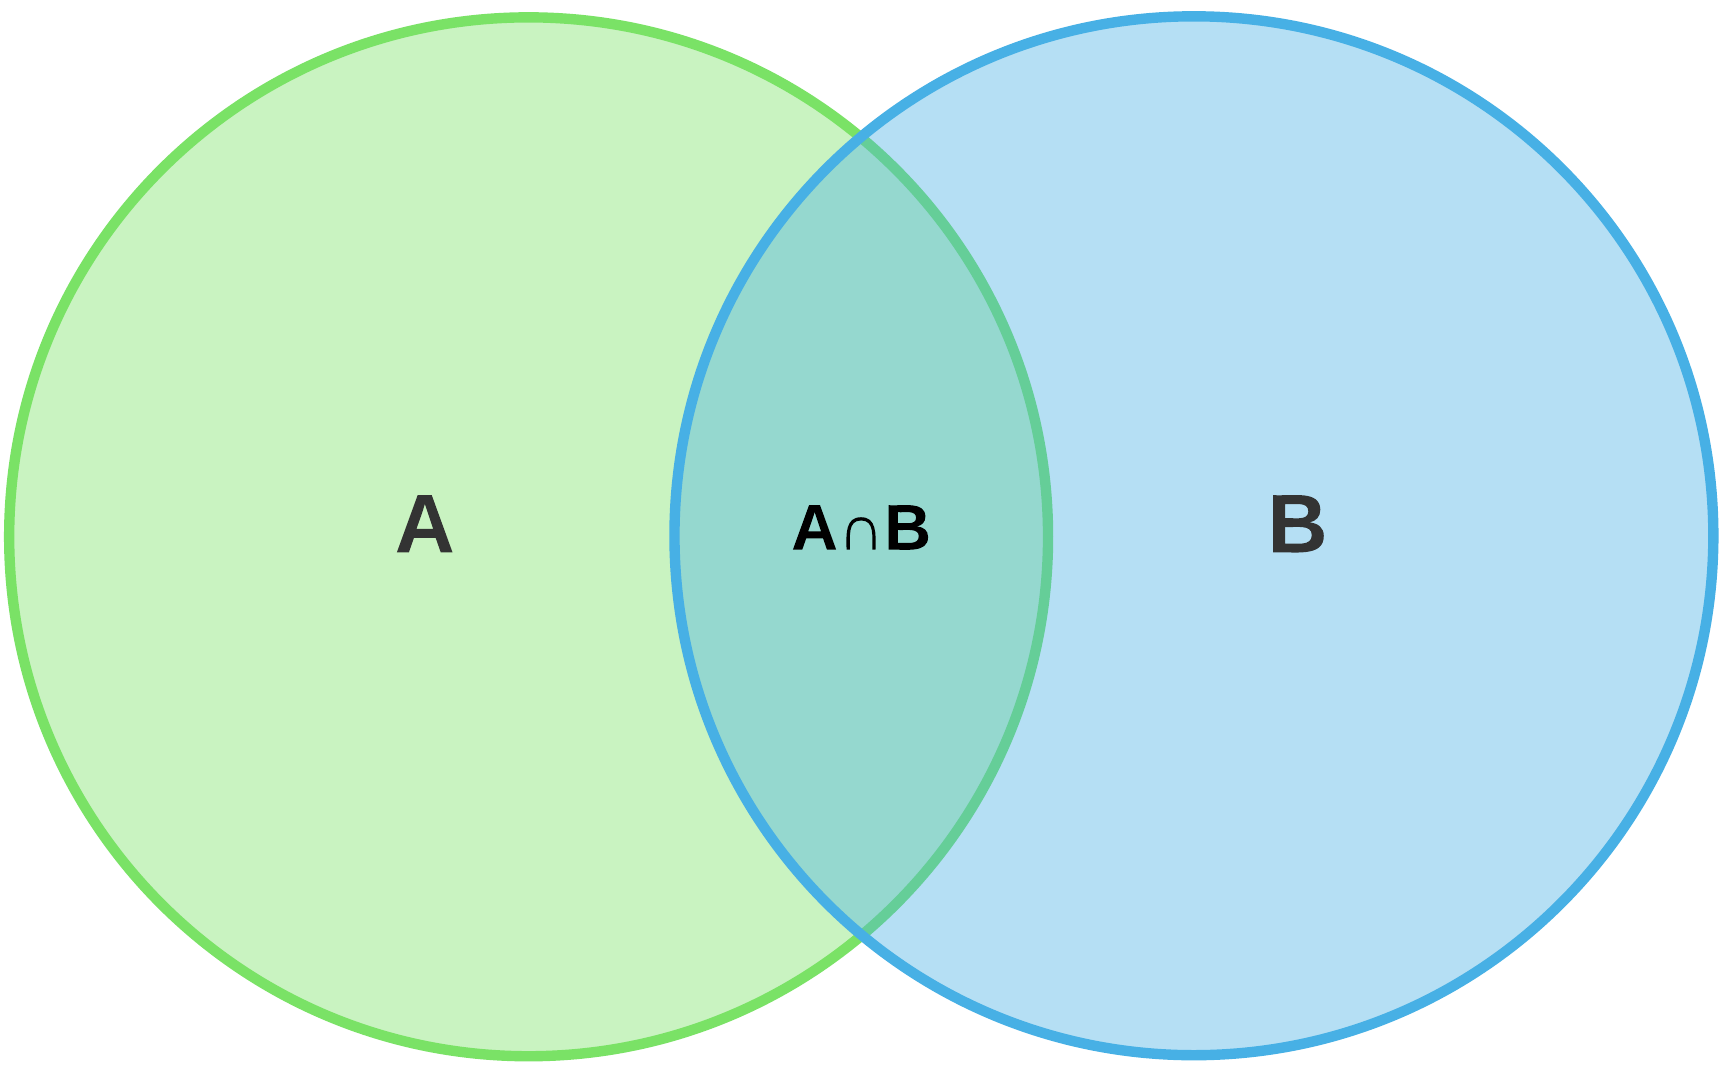
\includegraphics[width=0.4\textwidth]{venn.png}}
    \caption{Example of a Venn diagram representing the intersection of two sets $A$ and $B$.}
\end{figure}

\begin{remark}
    For any set $A,\quad A\cap\mathcal{U} = A,\quad\mathcal{U}\cup A = \uset$.
\end{remark}
\begin{definition}
    \textbf{(Complement of a set).} The complement of a set $A$ is another set such that
    \begin{equation}
        A^C:=\{a\in\uset\tq a\notin A\}
    \end{equation}
\end{definition}
\begin{example}
    Let $\uset = \Z$, then
    \begin{equation}
        \N\subset\uset, \quad\quad\N^C = \{x\in\Z\tq x<0\}
    \end{equation}
\end{example}

\begin{proposition}
\textbf{(De Morgan's laws)}. Let $A$ and $B$ be two sets in $\uset$. Then, the following equalities are hold.
\begin{equation}\label{demorgan:1}
    \left( A\cup B \right)^C = A^C\cap B^C
\end{equation}
\begin{equation}\label{demorgan:2}
    \left( A\cap B \right)^C = A^C\cup B^C 
\end{equation}
\end{proposition}
\begin{proof}
    \textit{(First De Morgan's law)}. In order to proof the first De Morgan's law we need first to proof that $\left( A\cup B \right)^C\subset A^C\cap B^C \textrm{ and then } A^C\cap B^C \subset \left(  A\cup B\right)^C$. Only then we can say $\left( A\cup B \right)^C = A^C\cap B^C $. 
    %Let $a\in\left( A\cup B \right)^C,\ a\in A^C\cap B^C$ ? So we take
    \begin{align}
        \textrm{Let } a\in\left( A\cup B \right)^C &\implies a\in\uset\textrm{ and } a\notin A\cup B \implies \\
                                     &\implies a\in\uset\textrm{ and } a\notin A\textrm{ and } a\notin B \implies \\ &\implies a\in A^C\textrm{ and } a\in B^C \implies \\
                                                         &\implies a\in A^C\cap B^C
    \end{align}
    So, we can afirm that $\left( A\cup B \right)^C \subset A^C\cap B^C $.
    \begin{align}
        \textrm{Now, let } b\in A^C\cap B^C &\implies b\in A^C\textrm{ and } b\in B^C \implies \\
                                            &\implies b\in\uset\textrm{ but } a\notin A\textrm{ and } a\notin B \implies \\ &\implies b\in\uset\textrm{ and } b\notin A\cup B \implies \\
                                            &\implies b\in \left( A\cup B \right)^C
    \end{align}
    So, we can afirm that $A^C\cap B^C\subset\left( A\cup B \right)^C $. Therefore,
    \begin{equation}
        \left( A\cup B \right)^C = A^C\cap B^C
    \end{equation}

\end{proof}

\begin{proof}
    \textit{(Second De Morgan's law)}. In order to proof the second De Morgan's law we need first to proof that $\left( A\cap B \right)^C\subset A^C\cup B^C \textrm{ and then } A^C\cup B^C \subset \left(  A\cap B\right)^C$. Only then we can say $\left( A\cap B \right)^C = A^C\cup B^C $. 
    %Let $a\in\left( A\cup B \right)^C,\ a\in A^C\cap B^C$ ? So we take
    \begin{align}
        \textrm{Let } a\in\left( A\cap B \right)^C &\implies a\in\uset\textrm{ and } a\notin A\cap B \implies \\
                                     &\implies a\in\uset\textrm{ and } a\notin A\textrm{ or } a\notin B \implies \\ &\implies a\in A^C\textrm{ or } a\in B^C \implies \\
                                                         &\implies a\in A^C\cup B^C
    \end{align}
    So, we can afirm that $\left( A\cap B \right)^C \subset A^C\cup B^C $.
    \begin{align}
        \textrm{Now, let } b\in A^C\cup B^C &\implies b\in A^C\textrm{ or } b\in B^C \implies \\
                                            &\implies b\in\uset\textrm{ but } a\notin A\textrm{ or } a\notin B \implies \\ &\implies b\in\uset\textrm{ and } b\notin A\cap B \implies \\
                                            &\implies b\in \left( A\cap B \right)^C
    \end{align}
    So, we can afirm that $A^C\cup B^C\subset\left( A\cap B \right)^C $. Therefore,
    \begin{equation}
        \left( A\cap B \right)^C = A^C\cup B^C
    \end{equation}

\end{proof}

\subsection{Partitions of sets}
\begin{definition}
    \textbf{(Partition of a set).} Let $A$ be a non-empty set. A partition of $A$ is a separation of $A$ into mutually disjoint non-empty subsets.
\end{definition}
\begin{example}
    Let $A = \{a, b, c, d, e\} $. A partition of $A$ could be
    \begin{equation}
        B_1 = \{a\}, \quad B_2 = \{b, e, d\}, \quad\ B_3 = \{c\}, \quad\quad B_1\cup B_2\cup B_3 = A
    \end{equation}
    \begin{equation}
        B_i\cap B_j = \O\quad\textrm{for}\quad i\neq j,\quad\quad B_i\neq\O\quad\textrm{for}\quad i = 1, 2, 3
    \end{equation}
\end{example}

\subsection{Other operations with sets}
\begin{definition}
    \textbf{(Difference of sets).} Let $A$ and $B$ be two sets. The difference of $A$ and $B$ is another set, $A\textbackslash B$, whose elements are the elements in $A$ which are not contained in $B$. 
    \begin{equation}
        A\textbackslash B := \{a\in A \tq a\notin B \} 
    \end{equation}
\end{definition}
\begin{definition}
    \textbf{(Symmetric difference of sets).} Let $A$ and $B$ be two sets. The symmetric difference of $A$ and $B$ is another set, $A\triangle B$, whose elements in $A$ that are not contained in $B$ and the elements in $B$ that are not contained in $A$.
    \begin{equation}
        A\triangle B := \{a\in A\tq a\notin B \}\cup \{b\in B\tq b\notin A \}  
    \end{equation}
\end{definition}
\begin{remark}
    $A\triangle B = A\cup B \textbackslash A\cap B$.
\end{remark}
\begin{example}[Let $A = \{1, 2, 3, 4\} $ and $B = \{3, 5, 7\} $.]
    \begin{equation}
        A\textbackslash B = \{1, 2, 4\} 
    \end{equation}
    \begin{equation}
        A\triangle B = \{1, 2, 4\}\cup \{5, 7\} = \{1, 2, 4, 5, 7\}   
    \end{equation}
\end{example}

\begin{proposition}
    $B\triangle A = \left( A\cap B \right)^C $.
\end{proposition}
\begin{proof}
    Let $A = \{a, b, c\} $ and $B = \{c, d\} $. Consider $\uset = A\cup B$.
    \begin{align}
        B\triangle A &= \{d\}\cup \{a, b\} = \{a, b, d\} \\
        A\cap B &= \{c\} \quad\rightarrow\quad \left( A\cap B \right)^C = \{a, b, d\} 
    \end{align}
    Therefore, the equality $B\triangle A = \left( A\cap B \right)^C $ is hold considering $\uset = A\cup B$.
\end{proof}

\begin{definition}
    \textbf{(Cartesian product of sets).} Let $A$ and $B$ be two sets. The cartesian product of $A$ and $B$ is the set of the ordered pairs of the form $\left( a, b \right)$ where $a\in A$ and $b\in B$.
    \begin{equation}
        A\times B := \{\left( a, b \right) \tq a\in A,\ b\in B\} 
    \end{equation}
\end{definition}

\begin{example}[Let $A = \{a, b, c\} $ and $B = \{c, 3\} $.]
    \begin{equation}
        A\times B = \{\left( a, c \right), \left( a, 3 \right), \left( b, c \right), \left( b, 3 \right), \left( c, c \right), \left( c, 3 \right)\}
    \end{equation}
\end{example}
\begin{note}
    In general, $B\times A\neq A\times B$.
\end{note}

\begin{definition}
    \textbf{(Cardinality of a set).} Let $A$ and $B$ be two sets. The cardinality of $A$, $\textrm{card}\left( A \right) $, is the number of elements in $A$.
    \begin{equation}
        \textrm{If card}\left( A \right) < \infty\textrm{ and } \textrm{card}\left( B \right) < \infty \implies \textrm{card}\left( A\times B \right) = \textrm{ card}\left( A \right)\cdot \textrm{ card}\left( B \right)   
    \end{equation}
\end{definition}

\subsection{Definition of a function}
\begin{definition}
    \textbf{(Function).} Let $X$ and $Y$ be two non-empty sets. The \textbf{function}, or \textbf{map}, from $X$ to $Y$ is a subset $f$ of $X\times Y$ such that for each $x\in X$ that appears as part of a pair in $f$, there is one, and only one $y\in Y$ such that $\left( x, y \right)\in f$, and we write $f:X\to Y$.
\end{definition}
\begin{example}[An example of a function would be]
    \begin{align}
        f:\R&\to\R \quad\quad\quad\quad\quad f = \{( x, x^2 + 1)\tq x\in\R \}\subset\R\times\R = \R^2 \\ 
        x&\to x^2 + 1
    \end{align}
\end{example}
\begin{example}[A typical non-example of a function would be]
    \begin{equation}
        h:=\{( x,\ \pm \sqrt{x})\tq x\in\R \}\subset\R\times\R = \R^2 
    \end{equation}
    \begin{itemize}
        \item If $x < 0$ then $\pm\sqrt{x} \notin\R $.
        \item We would have two inputs for the very same input value: 
            \begin{equation}
                (2, \sqrt{2} )\in h,\ ( 2, -\sqrt{2})\in h
            \end{equation}
    \end{itemize}
\end{example}
\begin{definition}
    Let $f:X\to Y$ and let $g:X\to Y$ be two functions. We say that $f = g$ if $\forall x\in X,\ f\left( x \right) = g\left( x \right)$.
\end{definition}

\subsection{Domain, codomain and range of a function}
\begin{definition}
    Let $f:X\to Y$ be a function. Then, 
    \begin{itemize}
        \item $X$ is the \textbf{domain} of the function: the set containing all the input values of the function. Since a function is defined on its entire domain, its domain coincides with its domain of definition.
        \item $Y$ is the \textbf{codomain} of the function: the set containing all of the output values of the function.
        \item The \textbf{range} of the function is the subset of $Y$:
            \begin{equation}
                \textrm{Range }:=\{y\in Y\tq \exists\ x\in X \textrm{ with } f\left( x \right) = y\} 
            \end{equation}
    \end{itemize}

    %\begin{itemize}
    %    \item $A$ is the \textbf{domain} of the function.
    %    \item $B$ is the \textbf{codomain} of the function.
    %    \item The \textbf{range} of the function is the following subset of $B$:
    %        \begin{equation}
    %            \textrm{range }:=\{b\in B\tq \exists\ a\in A \textrm{ with } f\left( a \right) = b \} 
    %        \end{equation}
    %\end{itemize}
\end{definition}
\begin{notation}
    The range of a function $f$ is often denoted by $f\left( A \right) $ or by Im$f$, which stands for \textit{image of $f$}.
\end{notation}

\subsection{Image and inverse image}
The word \textit{image} is used in three related ways. In these definitions, $f:X\to Y$ is a function from the set $X$ to the set $Y$.
\begin{definition}
    \textbf{(Image of an element).} If $x\in X$, then the image of $x$ under $f$, denoted $f\left( x \right) $, is the value of $f$ when applied to $x$.
\end{definition}
\begin{note}
    $f\left( x \right) $ is alternatively known as the output of $f$ for argument $x$.
\end{note}
\begin{definition}
    \textbf{(Image of a subset).} The image of a subset $S\subset X$ under $f$, denoted $f\left( S \right) $, is the subset of $Y$ which can be defined as follows:
    \begin{equation}
        f\left( S \right) := \{f\left( s \right) \tq x\in S\} 
    \end{equation}
\end{definition}
\begin{definition}
    \textbf{(Image of a function).} The \textbf{image} of a function is the image of its entire domain, also known as the range of the function.
\end{definition}

\hide{
\begin{definition}
    \textbf{(Image).} Let $f:X\to Y$ be a function and let $S\subset X$ be a subset. Then,
    \begin{equation}
        f\left( S \right):=\{y\in Y\tq \exists\ s\in S\textrm{ with } f\left( s \right) = y \}  
    \end{equation}
\end{definition}
}

\subsection{Surjective, injective and bijective functions}
\begin{definition}
    \textbf{(Surjective function).} A function $f$ from a set $X$ to a set $Y$ is \textbf{surjective} (also known as \textbf{onto}), if for every element $y$ in the codomain $Y$ of $f$, there is at least one element $x$ in the domain $X$ of $f$ such that $f\left( x \right) = y$. In other words, a surjective function is a function whose image is equal to its codomain. Symbolically,
    \begin{equation}
        \textrm{If } f:X\to Y\textrm{, then $f$ is said to be surjective if } \forall\ y\in Y,\ \exists\ x\in X \tq f\left( x \right) = y.   
    \end{equation}
\end{definition}
\begin{remark}
    It's not required that $x$ be unique; the function $f$ may map one or more elements of $X$ to the same element of $Y$.
\end{remark}
\begin{note}
    The French word \textit{sur} means \textit{over} or \textit{above}, and relates to the fact that the image of the domain of a surjective function completely covers the function's codomain.
\end{note}
\begin{notation}
    If $f:X\to Y$ is such that $f\left( x \right) = y$ we say that $y$ is the image of $x$ by $f$ and we'll say that $x$ is the preimage of $y$ by $f$.
\end{notation}
\begin{figure}[htbp]
    \centerline{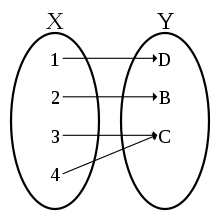
\includegraphics[width=0.25\textwidth]{surjective-function.png}}
    \caption{A surjective function from domain $X$ to codomain $Y$.}
\end{figure}
\begin{definition}
    \textbf{(Injective function).} Let $f$ be a function whose domain is a set $X$. The function $f$ is said to be \textbf{injective} (or \textbf{one-to-one}), provided that for all $a$ and $b$ in $X$, whenever $f\left( a \right) = f\left( b \right)$, then $a = b$. Symbolically,
    \begin{equation}
        \textrm{If } f:X\to Y\textrm{, then $f$ is injective if }\forall\ a, b\in X,\ f\left( a \right) = f\left( b \right) \implies a = b.
    \end{equation}
\end{definition}
\begin{figure}[htbp]
    \centering
    \begin{subfigure}{.25\textwidth}
        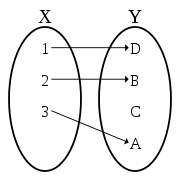
\includegraphics[width=\textwidth]{injective-nonsurjective-func.png}
        %\caption{An injective non-surjective function.}
    \end{subfigure}
    \hspace{1cm}
    \begin{subfigure}{.25\textwidth}
        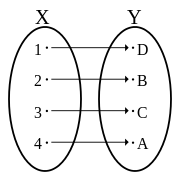
\includegraphics[width=\textwidth]{injective-surjective-func.png}
        %\caption{An injective surjective function.}
    \end{subfigure}
    %\centerline{\includegraphics[width=0.3\textwidth]{injective-function.png}}
    \caption{Injective non-surjective function (left) / Injective surjective function (right).}
\end{figure}

\begin{definition}
    \textbf{(Bijective function).} Let $f$ be a function from a set $X$ to a set $Y$. The function $f$ is said to be \textbf{bijective} if it's both surjective and injective. In other words, each element of one set is paired with exactly one element of the other set, and each element of the other set is paired with exactly one element of the first set.
\end{definition}

\begin{remark}
    If $X$ and $Y$ are finite sets, then the existence of a bijection means they have the same number of elements.
\end{remark}
\begin{figure}[htbp]
    \centerline{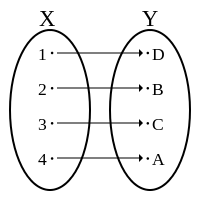
\includegraphics[width=0.25\textwidth]{bijective-func.png}}
    \caption{A bijective function, $f:X\to Y$.}
\end{figure}

A bijective function from the set $X$ to the set $Y$ has an \textbf{inverse function} from $Y$ to $X$.

\newpage
\begin{definition}
    \textbf{(Inverse function).} Let $f$ be a function whose domain is the set $X$, and whose codomain is the set $Y$. Then, $f$ is \textbf{invertible} if there exists a function $g$ with domain $Y$ and image $X$, with the property
    \begin{equation}
        f\left( x \right) = y \iff g\left( y \right) = x
    \end{equation}
\end{definition}

If $f$ is invertible, then the function $g$ is unique, which means that there is exactly one function $g$ satisfying this property. That function $g$ is then called the \textbf{inverse} of $f$, usually denoted as $f^{-1}$.
\begin{proposition}
    If $f$ is an invertible function with domain $X$ and range $Y$, then
    \begin{equation}
        f^{-1}\left( f\left( x \right)  \right) = x,\quad \forall\ x\in X.
    \end{equation}
\end{proposition}
\begin{example}[.]
    Let $g:\R\to\R$ be a bijective function which $x\mapsto 2x + 1$. In order to calculate the inverse $g^{-1}:\R\to\R$ of the bijective function $g$ we should write the function in terms of $y$ and then change $y$ for $x$.
    \begin{equation}
        2x + 1 = y \quad\iff\quad x = \frac{y - 1}{2} \quad\rightarrow\quad g^{-1} = y = \frac{x - 1}{2}
    \end{equation}
    \begin{align}
        g^{-1}:\R&\to\R \\ x&\mapsto \frac{x - 1}{2}
    \end{align}
\end{example}

